\firstsection{Introduction} 
\maketitle
%目前,有一个多维数据分析领域中的新兴热门话题,自动化地传递见解,它能有效地降低了用户在探索数据中的努力,通过自动的见解发现,精心设计的布局和叙事结构,和引人入胜的可视映射。这些优点促进了自动传递见解创作工具的快速发展,例如datashot,data videos, 和calliope。上述的工作把用户从创作中解放出来,让他们更专注于高层的探索,这对于缺乏创作领域知识的普通受众是友好的,能够促进可视分析工具的普及。表格数据作为常见的信息存储介质,被选为本工作的关注点。在接下来的讨论中,我们用数据事件来表示表格数据中见解。
Currently, automatic insight delivery is emerging as a promising visual analysis approach in multi-dimensional data exploration. 
This technique can effectively reduce the effort of users in exploring data, through automatic insight discovery, well-designed layout and narrative structure, and engaging visual mapping. 
More and more researchers are attracted to create authoring tools for automated delivery of insights, such as datashot, data videos, and calliope. 
These tools liberate users from creation and allows them to focus on high-level exploration, that is friendly to ordinary audiences who are lack of domain-specific knowledge, and promotes the popularization of visual analysis tools.
Tabular data, as a common information storage medium, is selected as the focus of this work. In the following discussion, we utilize data fact to represent the insight in tabular data.

%根据一些评估指标来排序自动提取的见解并选择前top-k,是上述工作常采用的见解挖掘方法。然而,这样会导致大量的见解不可见。尽管这些事件在评估有不好的表现,但这不能定论他们在辅助用户理解中的作用。由于技术的限制,有一些见解难以被探查,如图中蓝色框外的圆点所示。和之前的工作相同,提升事件的检测能力目前不是我们的关注点。本工作更关注用户对事件空间的理解力以及他们能否有效顺利地定位到符合需求的事件。此外,上述方法的另一个局限是丢失了top-k见解的上下文信息,这不利于不同见解之间的过渡。总之,本工作面临的第一个挑战就是事件空间的概览以及支撑事件的上下文关系。
Ranking the data facts according to certain evaluation metrics and selecting the top-k ones is a common fact delivery approach utilized in aforementioned works. 
However, this will make a large number of facts invisible. Although these facts have a poor performance in the evaluation, it is not conclusive that their role in aiding users understanding.
Due to technical limitations, there are certain hard-to-find facts, as shown by the outermost dots in figure \ref{factspace}. 
As with the existing work, improving the fact detection ability is not our focus. This work focuses more on users' understanding of the fact space and whether they can effectively and smoothly locate the ones that meet their needs (dots in orange boxes in figure \ref{factspace}).
Furthermore, another limitation of the aforementioned approach is that the contextual information of the top-k facts is also lacking, which is not beneficial for users to switch between different facts.
In summary, the first challenge of this work is to support an overview of the whole fact space, as well as the context of each fact.

%数据故事将事件组装进精心设计的叙事结构已生成有意义的事件序列,是一种更加有效的传递见解的途径。已有工作针对研究如何构建优质的叙事序列,如xxxxxxxx。之前工作生成的故事线往往是在规则和评估表现最优的,但是这样的故事线视角单一和思考模式固定,留给用户的探索性不足。用户只能顺着算法最优的思考模式获取信息,而不是主动地按照自己的思考模式去探索。探索型的叙事不仅能够增强用户的趣味性还能揭露潜在的一些模式。本工作第二个挑战就是如何从多视角地生成故事线,增强用户探索的自主性,让用户能够决定叙事走向。
Data story, which assembles fact pieces into well-designed narrative structure to generate a meaningful sequence, is a more effective approach of delivering insights. 
Existing work has focused on researching how to construct high-quality narrative sequences. Such as,
Calliope incorporates a logic-oriented Monte Carlo tree search algorithm to progressively generate data facts and organize them in a logical sequence. 
Storylines, which generated in previous work, generally have good performance in evaluation or rule constraints. However, such storylines usually have a single narrative perspective and a fixed mindset, and can not provide a flexible exploration. 
Users can only receive information in the mindset that perform well in algorithm evaluation, instead of independently exploring according to their own mindset. 
Exploratory narratives can make user exploration more interesting and reveal more underlying patterns. 
Thence, the second challenge of this work is how to generate storylines from multiple perspectives, enhance the autonomy of exploration, and allow users to decide the direction of the narrative.
\begin{figure}[t]
	\centering
	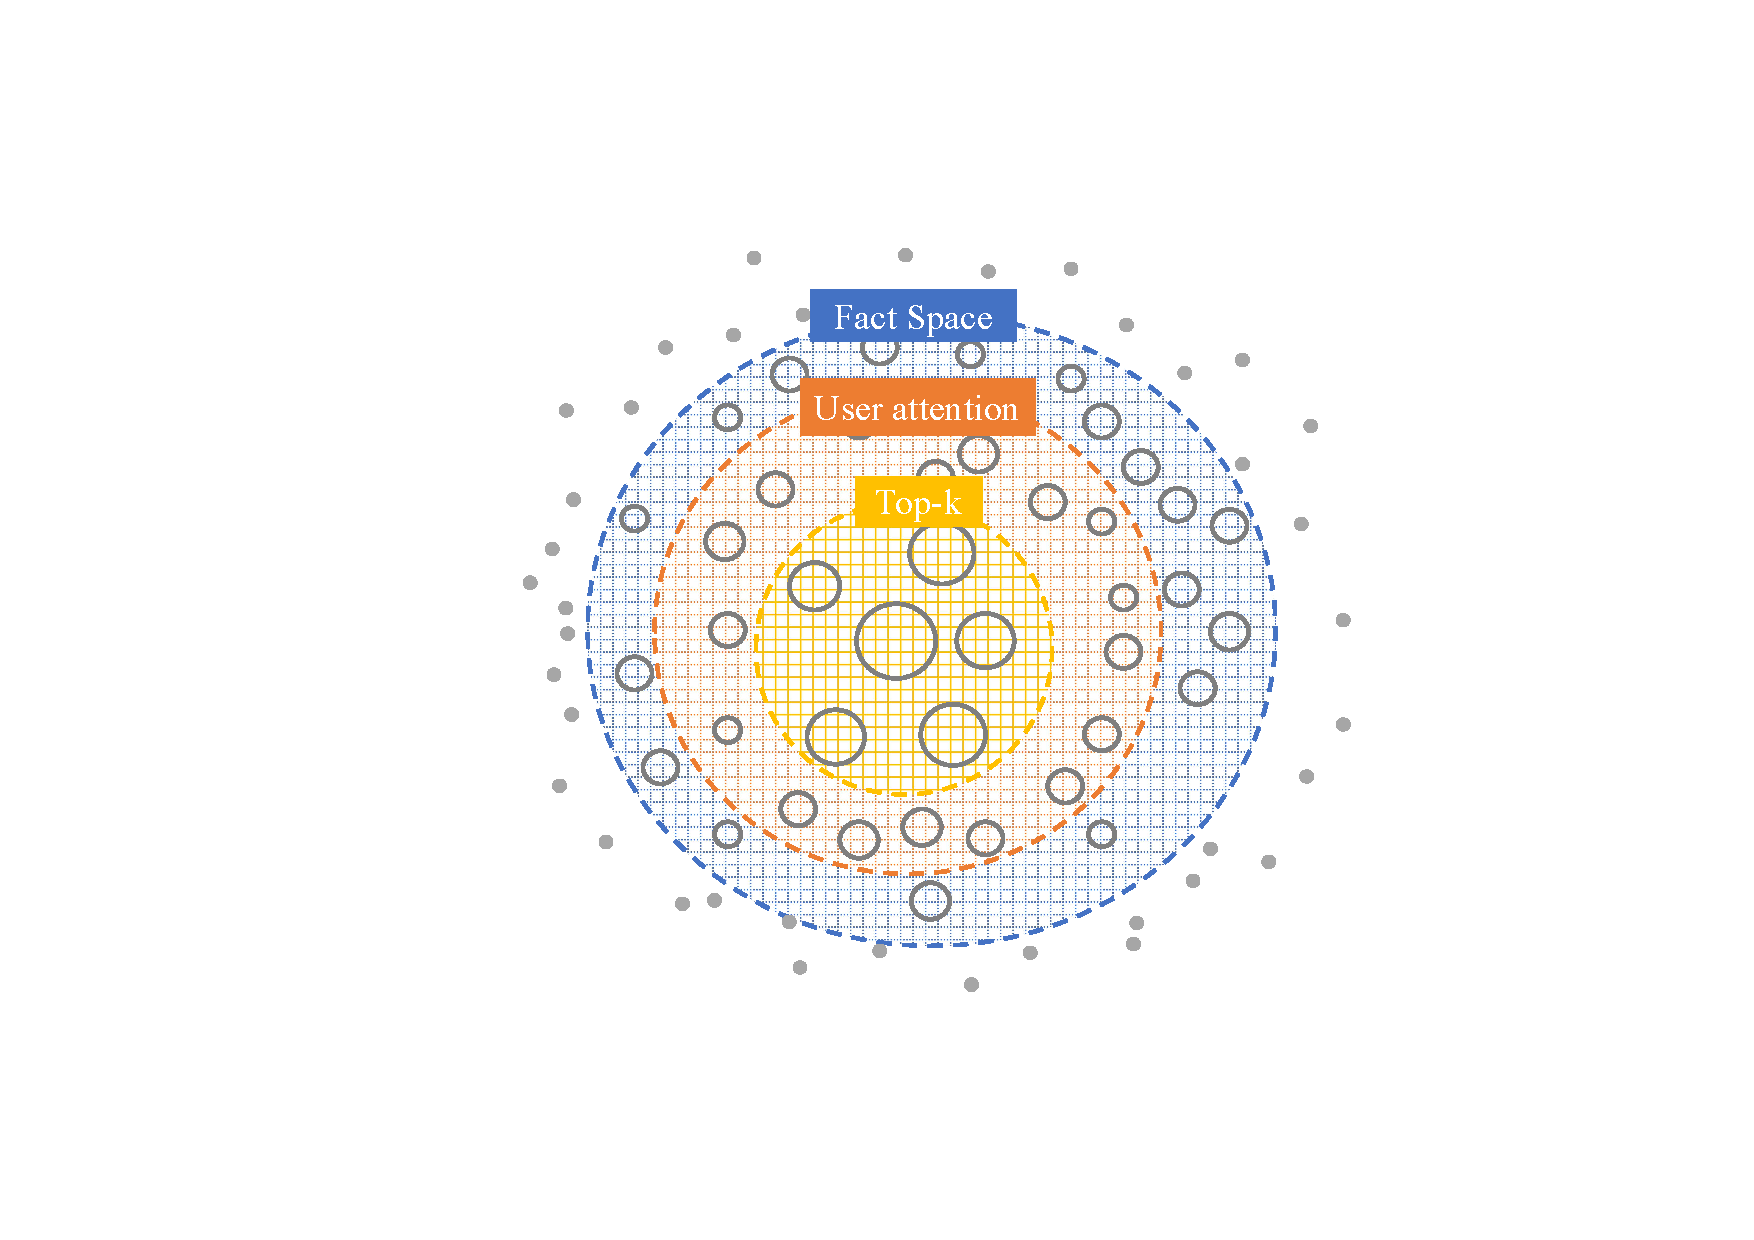
\includegraphics[width=0.5\textwidth]{figures/introduction.pdf}
	\caption{The illustration of fact space. The dots in blue box are the facts automatically extracted, orange box includes the facts that may be of interest to users, and top-k facts are in yellow box }
	\label{factspace}
\end{figure}

%为了解决上述挑战,我们提出了一个辅助探索事件空间的框架,框架由事件提取、事件嵌入和故事线提取三部分组成。我们引入了一种能够衡量数据事件相似性的双因素嵌入方法来将事件嵌入事件空间。一个新颖的变分编码器被采用来嵌入事件的视觉编码信息,根据之前的调查研究结果计算事件之间的逻辑距离来嵌入事件的逻辑信息。此外,我们还设计了一种新颖的多视角故事线生成算法。该算法分别从top-k个fact出发拓展故事线。一个事件路径搜索算法也被设计来寻找两个事件之间的过渡路径。最后,这些想法被实现在了一个用于探索事件空间的系统,FactExplorer。在系统中,我们还为用户设计了许多的交互通道,运行用户便捷地编辑事件和事件故事线。本文的主要贡献如下:
To address the above challenges, we propose a framework to assist in exploring the fact space, which consists of three parts: fact extraction, fact embedding, and storyline generation. 
In the fact embedding module, we introduce a two-factor embedding approach, which can measure the similarity of data facts, to embed facts into the fact space. 
More specifically, a novel variational encoder is employed to encode the visual style details of facts, and the logical relation of facts is embedded by computing the logical distance among facts based on the findings from previous work. 
Furthermore, we design a novel multi-storyline generation algorithm, which expands multi-perspective storylines from top-k facts respectively. A fact path search algorithm is also designed to seek a smooth and informative transition path from one fact to another.
Finally, these ideas are implemented in a fact space exploration system, FactExplorer. 
Certain interactions are also provided in the system to support flexible editing of facts and fact storylines.
The major contributions of this paper are as follows:
\begin{itemize}
%一个名为FactExplorer的可运行的系统,被设计来自动地挖掘表格数据背后的事件空间。合适的交互组件在系统中也被提供来支持灵活高效的探索
\item A runnable system named FactExplorer is designed to automatically build a fact space from tabular data. Appropriate interaction components are also provided in the system to support flexible and efficient exploration.
%一个用来将事件嵌入到事件空间的双因素(可视化样式和逻辑性)事件嵌入的方法。一个新颖的变分编码器模型被采用来嵌入可视化样式,逻辑性嵌入则通过计算事件之间的逻辑距离来实现,最后将它们聚合起来。
\item A two-factor (visual style and logical) fact embedding approach for embedding facts into the event space. A novel variational encoder model is utilized to embed visual styles, and logical embedding is achieved by computing the logical distance among facts, and finally aggregate these results to get fact embedding vector.
%一个多视角故事线生成算法来便捷用户的探索和增强用户对事件空间的记忆
\item An exploratory narrative approach is proposed to improve the flexibility and interest of exploration. More specifically, a multi-storyline generation algorithm is designed to generate multi-perspective storylines. A fact path search algorithm is also designed to seek a smooth and informative transition path from one fact to another.
\end{itemize}